\documentclass[letter,12pt]{article}
\usepackage{jheppub}
\usepackage{taro}
\usepackage{booktabs}

\usepackage{mathrsfs}
\usepackage{tcolorbox}
\newcommand{\red}[1]{\textcolor{red}{#1}}
\newcommand{\pink}[1]{\textcolor{pink}{#1}}
\newcommand{\blue}[1]{\textcolor{blue}{#1}}
\newcommand{\green}[1]{\textcolor{ForestGreen}{#1}}
\newcommand{\orange}[1]{\textcolor{orange}{#1}}
\newcommand{\brown}[1]{\textcolor{brown}{#1}}

\newcommand{\J}{\mathcal{J}}
\newcommand{\BO}{\mathcal{O}}
\newcommand{\OO}{\mathcal{O}}

\newcommand{\ab}[1]{\langle #1 \rangle}
\newcommand{\sqb}[1]{[ #1 ]}
\newcommand{\aMs}[3]{\langle #1|#2|#3]}  		% <1|2|3]
\newcommand{\aMMa}[3]{\langle #1|#2|#3\rangle}		% <1|Q_1.Q_2|3>
\newcommand{\sab}[1]{s_{#1}}
\newcommand{\twhite}[1]{\textcolor{white}{#1}}

\title{Quantum Error Correction in AdS/CFT}

\def\Tr{{\rm Tr}}
\def\MHVbar{${\overline{\rm MHV}}$}
\def\nn{\nonumber}
\def\NeqFour{${\cal N}=4$}
\def\Split{{\rm Split}}
\def\spa#1.#2{\left\langle#1\,#2\right\rangle}
\def\spb#1.#2{\left[#1\,#2\right]}
\def\sandmx#1.#2.#3{%
	\left\langle#1{\vphantom1}\right|{#2}\left|#3\right]}%
\def\delt#1{\delta^{(#1)}}
\def\eps{\epsilon}
\def\Ord{{\cal O}}
\def\tlambda{\tilde\lambda}
\def\draftnote#1{{\sl #1}}
\def\tp{\!+\!}
\def\sA{{\cal A}}
\def\Int#1{I^{(#1)}}

\author[a]{Taro V. Brown}

\affiliation[a]{Department of Physics, UC Davis, One Shields Avenue, Davis, CA 95616, USA }


% e-mail addresses: one for each author, in the same order as the authors
\emailAdd{tvbrown@ucdavis.edu}


\abstract{a}

\begin{document} 
\maketitle
\flushbottom
\newpage
\section{Introduction}
The AdS/CFT correspondence is a duality relating a
$(d+1)$-dimensional bulk theory of gravity in anti-de Sitter spacetime (AdS) to a $d$-dimensional boundary conformal field theory (CFT). The importance of the duality can not be understated, as the mathematical structure, and especially ulta-violet (UV) behavior, is not fully understood on the gravity side, as opposed to the framework of CFT's, which has been studied for a long time. The duality therefore gives a path towards a theory of quantum gravity, or at least gives hints on certain properties that such a theory should have.

The correspondence provides a dictionary between the CFT and Gravity sides. The focus of this project is on how one relates operators on the boundary to operators in the bulk. This might seem strange at first, since the operators on the boundary live in one spacetime dimension lower than the bulks ones and so one might expect the dictionary to only work one way, but as we will show, one is able to \textit{reconstruct} information in the bulk from data on the boundary. Further, one can reconstruct operators using only part of the boundary information. Here we will focus on Rindler reconstruction, but other subregion dualities exist. 

Using Rindler reconstruction, some subtleties and puzzles in the prescription appear. We will describe the problems and then show how treating AdS/CFT as a Quantum Error Correcting Code (QECC), resolves the problems. For this purpose we introduce a toy model: the 3 qutrit model. The model is very coarse grained and we give a brief introduction to how to introduce more degrees of freedom by using tensor networks.
\section{Bulk and Rindler Reconstruction \label{sec:1}}
We are going to consider global AdS spacetime with metric
\begin{equation}
	\begin{aligned}
		\dd s^2=&-\left(1-r^2\right)\dd t^2+\left(1-r^2\right)^{-1}\dd r^2+r^2\,\dd\Omega_{d-1}^2
		\\
		=&\omega(\rho)^2\left(-\dd t^2+\dd \rho^2+\sin^2\rho\,\dd\Omega_{d-1}^2 \right),
	\end{aligned}
\end{equation}
where we work in natural units, such that the AdS length $\ell_{\text{AdS}}=1$ and we have defined $r\equiv \tan\rho $ as well as the the conformal factor $\omega(\rho)\equiv \frac{1}{\cos\rho}$ in the second line. This metric is conformally related to the Einstein Static Universe, and its conformal structure can be illustrated on a cylinder. The boundary is located at $r=\infty$ and can be viewed as the cylindrical shell of the global AdS space time.

We are going to denote bulk coordinates by $x\equiv (r,t,\Omega)$ and boundary coordinates by $X\equiv (t,\Omega)$. The AdS/CFT duality provides a map between operators on the boundary $\OO(X)$ and operators in the bulk $\phi(x)$. This is illustrated the global AdS cylinder on figure \ref{fig:adscftfig1}.
\begin{figure}[]
	\centering
	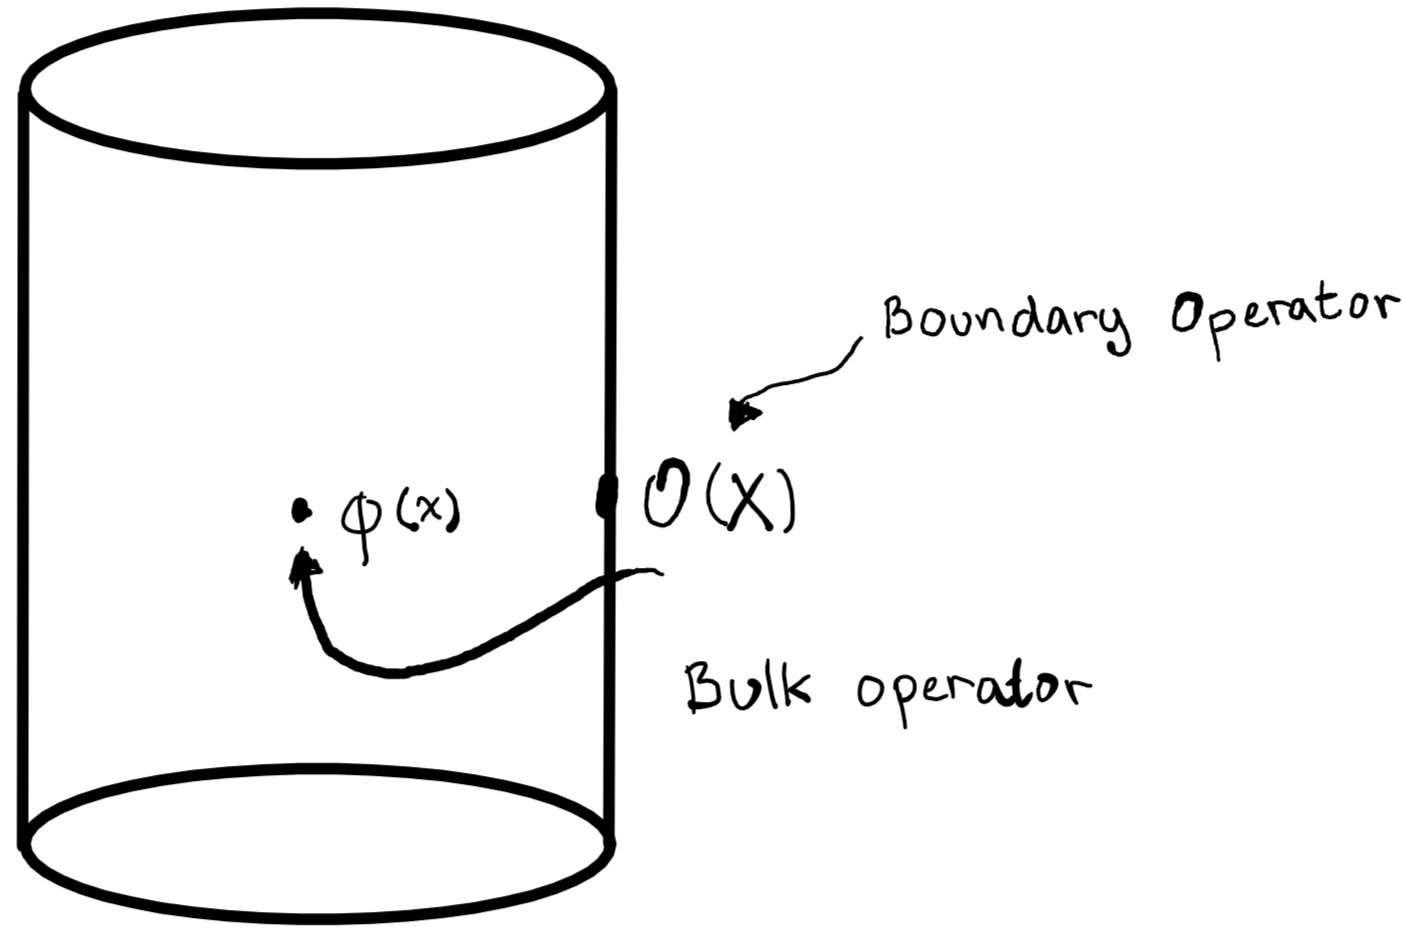
\includegraphics[width=0.6\linewidth]{ADS_CFT_Fig1}
	\caption{Global AdS as a cylinder with bulk operator $\phi(x)$ and boundary operator $\OO(X)$}
	\label{fig:adscftfig1}
\end{figure}
If one solves the equations of motion of the bulk field $\phi(x)$ near the boundary and demands that the solution is normalizable, the following extrapolate dictionary relates it to the boundary operator,
\begin{equation}
	\begin{aligned}
		\lim_{r\to \infty}r^{\Delta}\phi(x)=\BO(X)	\end{aligned}, \label{eq:1}
\end{equation}
where for a generic scalar of mass $m$, $\Delta$ satisfies $\Delta(\Delta-d)=m^2$. This limit seems very natural and one can ask whether it is possible to obtain the bulk solutions if the boundary operator is known. I.e. we are interested in the following 
\begin{equation}
	\begin{aligned}
		\phi(x)=\int\dd X K(x;X)\BO(X) \label{eq:2}
	\end{aligned}
\end{equation}
under the boundary condition \eqref{eq:1}. Here $ K(x;X)$ is a Greens function, often refered to as the \textit{smearing function}. If one takes a bulk point $x$, then $K(x;X)$ has support on set of boundary points that are spacelike separated from $x$, see Figure \ref{fig:adscftfig2}a. 

We are going to focus on constructing operators from boundary subregions. One such subregion is the Rindler wedge, $W$, defined by metric
\begin{equation}
	\begin{aligned}
		\dd s^2=-(\rho^2-1)\dd \tau^2+(\rho^2-1)^{-1}\dd \rho^2+\rho^2\dd H_{d-1}^2
	\end{aligned}
\end{equation}
with $\dd H^2_{d-1}=\dd \chi^2+\sinh^2\chi\dd \Omega_{d-2}^2$ is the metric on a $d-1$ dimensional hyperbolic ball. The metric has $\rho>1$ and $-\infty <\tau < \infty$ and its embedding in the global AdS cylinder is shown on Figure \ref{fig:adscftfig2}b. Using similar arguments to the global reconstruction, it can be shown explicitly that a bulk field can be reconstructed from a boundary operator if it lies within the Rindler wedge,
\begin{equation}
	\begin{aligned}
		\phi(x)|_{x\in W}=\int_{\partial W}\dd X K(x;X)\BO(X)
	\end{aligned}
\end{equation}
where $K(x;X)$ now only has support on the boundary region of the wedge. Using this as a jumping off point, we can find a version of \eqref{eq:2} for any subregion, using the causal wedge, $W_C$, for any boundary spatial subregion $A$ , defined by 
\begin{equation}
	\begin{aligned}
		W_C[A]=\mathscr{I}^+[D_\partial[A]]\cap\mathscr{I}^-[D_\partial[A]]
	\end{aligned}
\end{equation}
The bulk field can the be reconstructed on the boundary region $A$ as long as it is in the causal wedge, see Figure \ref{fig:adscftfig2}c. 
\begin{figure}[]
	\centering
	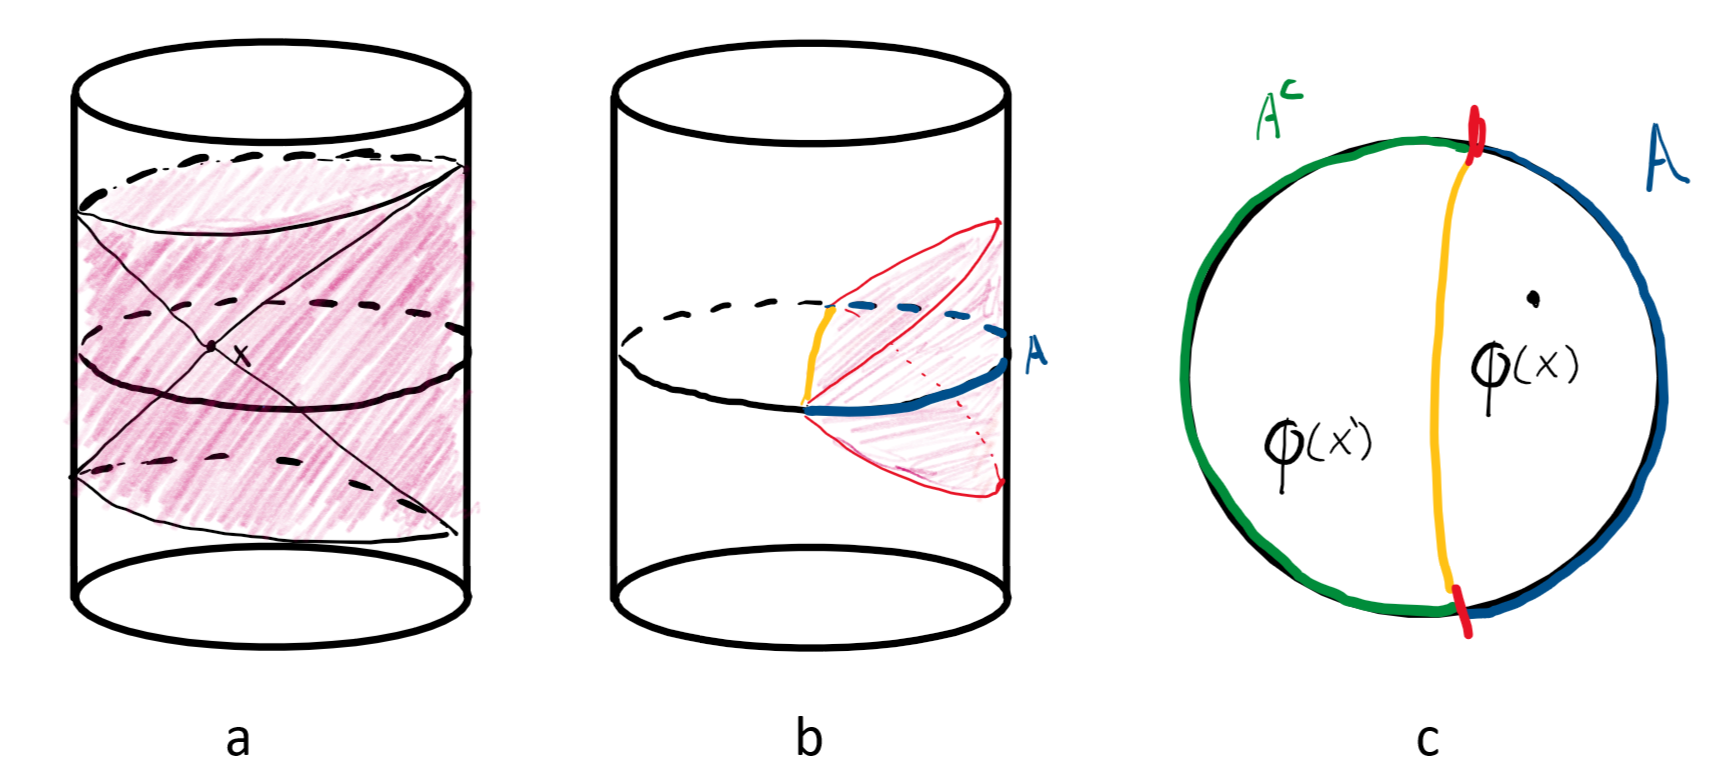
\includegraphics[width=0.95\linewidth]{ADS_CFT_Fig2}
	\caption{}
	\label{fig:adscftfig2}
\end{figure}
Using these definitions we arrive at two puzzles, which we will describe below.
\subsubsection*{Radial Commutivity Puzzle}
Using the reconstruction procedure just described on a t=0 timeslice with support on a region $A$ that covers almost the whole boundary region, as shown on Figure \ref{fig:adscftfig3}a, one finds that the operator dual to $\phi$ on the boundary, will necessarily commute with an operator $\OO$ that lies in the complement region $A^C$. 
\begin{equation}
	\begin{aligned}
		\left[\phi(x),\BO(X')\right]=0
	\end{aligned}
\end{equation}
Similarly one can pick a different operator $\OO '$ on the boundary and by using a new region $A'$, see Figure \ref{fig:adscftfig3}b, we once again find that $\phi$ commutes with $\OO '$. We can in fact do this with all operators and so must conclude that $\phi$ commutes with \textit{all} operators on the boundary.
\begin{figure}[]
	\centering
	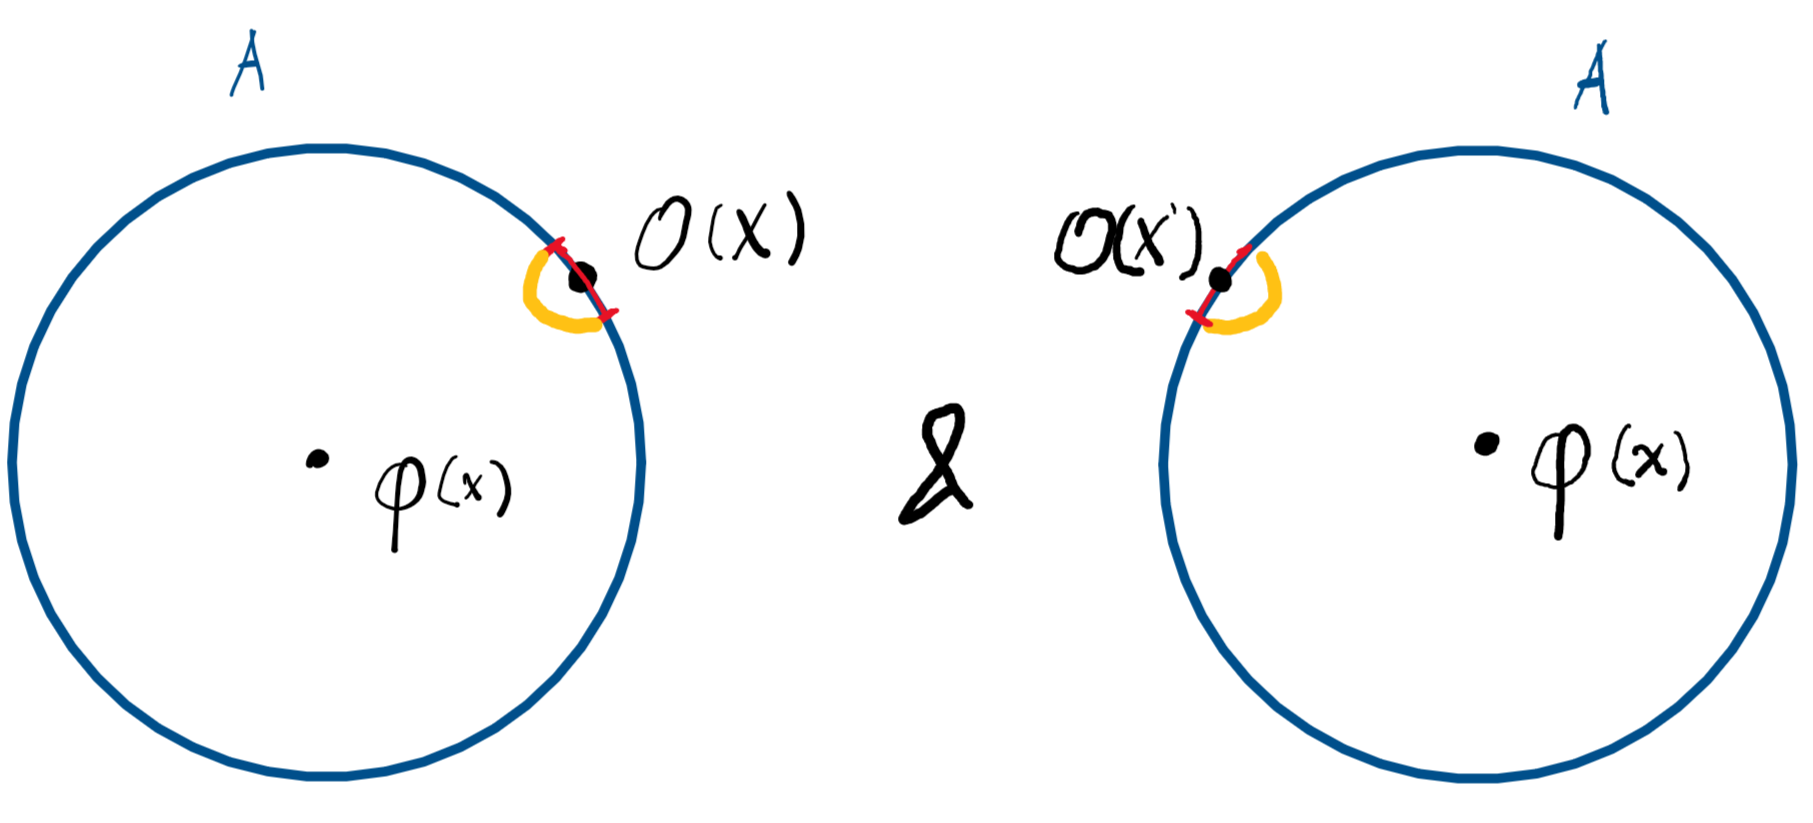
\includegraphics[width=0.75\linewidth]{ADS_CFT_Fig3}
	\caption{}
	\label{fig:adscftfig3}
\end{figure}
This however contradicts a well-known quantum field theory theorem known as the \textit{time-slice axiom}, which states that any operator which commutes with all local operators at a fixes time most be trivial. Since $\phi$ obviously is not trivial this is quite puzzling.

\subsubsection*{ABC Puzzle}
The ABC-puzzle is best illustrated through Figure \ref{fig:adscftfig4}. Using the reconstruction procedure $\phi$ can not be reconstructed on regions $A$, $B$, or $C$, it can however be reconstructed from any combination of two regions. So there exists at least 3 representation of $\phi$: $\phi_{AB},\; \phi_{BC},$ and $\phi_{CA}$. The can not be the same operator on the CFT however, and so we get yet another puzzle. 
\begin{figure}[]
	\centering
	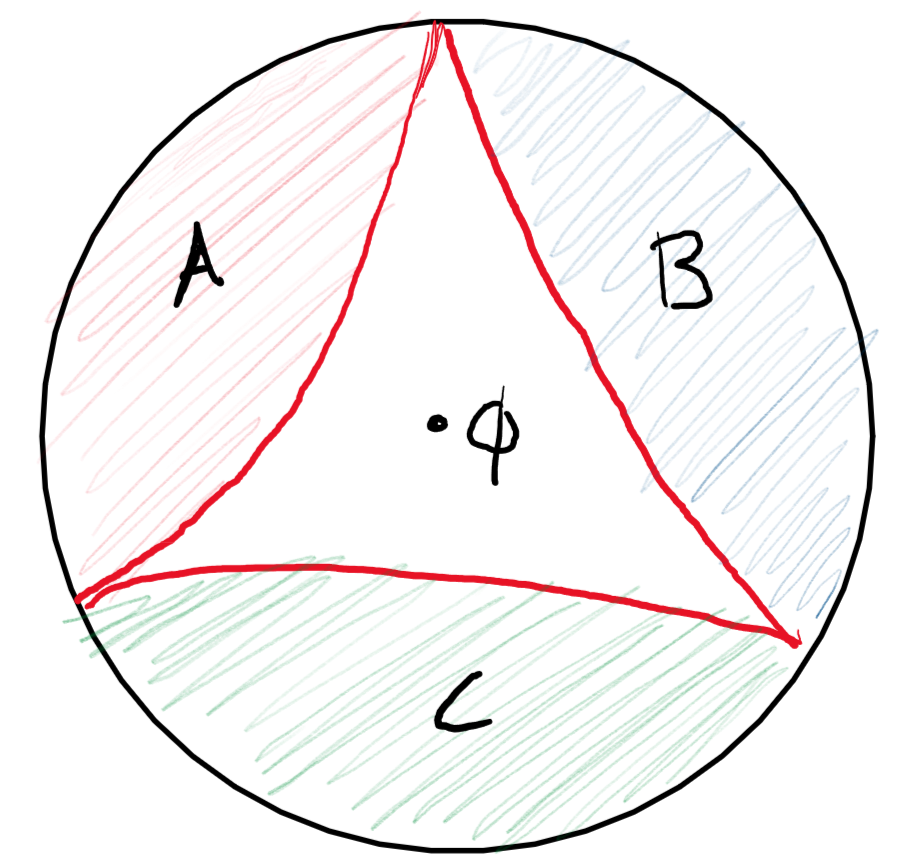
\includegraphics[width=0.25\linewidth]{ADS_CFT_Fig4}
	\caption{}
	\label{fig:adscftfig4}
\end{figure}

Both puzzles can however be resolved by interpreting the correspondence as an quantum error correcting code, which we will describe next.

\section{Quantum Error Correction - The Qutrit Model}
Error correction is the procedure off protecting information from being lost. The type of loss can be manifold, but if one is talking about quantum information it could e.g. be decoherence. 

In classical computers an easy way to protect information is through redundancy - simply sending your information multiple times. In quantum mechanics however, we are not able to procure our quantum bits (or, as we will see below, qutrits) in the same state due to the no-cloning theorem. Instead we have to come up with a new way to protect information. 

For this purpose we are going to define the 3-qutrit model. The qutrit is a 3 dimensional extension of the qubit (i.e. Bell state) and it has the basis $\{\ket{0},\ket{1},\ket{2}\}$. Using these, Alice wants to send a qutrit $\ket{\psi}$ to Bob
\begin{equation}
	\begin{aligned}
		\ket{\psi}=\sum_{k=0}^{2}c_k \ket{k}
	\end{aligned}
\end{equation}
We will refer to this as the \textit{logical qutrit}. She wants to do it in a way that preserves the original qutrit even if part of the information is lost. To do this she writes the information in terms of a 3-qutrit state:
\begin{equation}
	\begin{aligned}
		|\tilde \psi\rangle=\sum_{k=0}^{2}c_k \tilde{\ket{k}}
	\end{aligned}
\end{equation}
where the basis vectors now are
	\begin{equation} \label{eq:masslessSH}
		\begin{aligned}
			|\tilde 0\rangle &=\frac{1}{\sqrt{3}}\left(\ket{000}+\ket{111}+\ket{222}\right)\\
			|\tilde 1\rangle &=\frac{1}{\sqrt{3}}\left(\ket{012}+\ket{120}+\ket{201}\right)\\
			|\tilde 2\rangle &=\frac{1}{\sqrt{3}}\left(\ket{021}+\ket{102}+\ket{210}\right)\\
		\end{aligned}
	\end{equation}
such that $\left\{|\tilde k\rangle\right\}$ forms a basis for a 3-dimensional subspace, denoted by $H_{\text{code}}$ within the full 27 dimensional Hilbert space of the qutrits. The 3 qutrits encoding the information of the logical qutrit is called \textit{physical qutrits}. 

Before we move on, let us summarize some important features of the states just defined:
\begin{itemize}
	\item $H_{\text{code}}$ is symmetric under exhange of the 3 qutrits.
	\item All $| \tilde \psi \rangle\in H_{\text{code}}$ are highly entangled, since the density matrix obtained from tracing out two qutrits, i.e.
	\begin{equation}
		\begin{aligned}
			\rho_{\text{single qutrit}}=\frac{1}{\sqrt{3}}
			\left(\dyad{0}{0}+\dyad{1}{1}+\dyad{2}{2}\right)	\end{aligned}
	\end{equation}
is a maximally mixed state. 
\item Any single qutrit has no information about the original state.
\item Any two of the three qutrits contains complete information about the original state, so even if Bob looses a single qutrit he can still recover the original information. We will describe how this works below.
\end{itemize}
To see that the physical qutrits contain all the information from the logical qutrit, we define decoding operators $U_{ij}$, for $\{i,j\}=1,2,3$, $i\neq j$. It is easiest to see how these through an explicit example, so take e.g. $U_{12}$, which has the explicit action of changing the first two qutrits in the following manor,
\begin{align}
	\begin{tabular}{ l c r }
		$|00\rangle\to|00\rangle$ & $|11\rangle \to |01\rangle$ & $|22\rangle\to |02\rangle$ \\ 
		$|01\rangle \to |12\rangle$ & $|12\rangle \to |10\rangle$ & $|20\rangle \to |11\rangle$ \\
		$|02\rangle\to |21\rangle$ & $|10\rangle\to|22\rangle$ & $|21\rangle \to |20\rangle$ 
	\end{tabular}.
\end{align}
Such that, for instance acting on the $|\tilde 1\rangle$
\begin{equation}
	\begin{aligned}
		U_{12}|\tilde 1\rangle&=\frac{1}{\sqrt{3}}\left(\ket{122}+\ket{100}+\ket{111}\right)
		\\
		&=\ket{1}_1\otimes \ket{\chi}_{23}
	\end{aligned}
\end{equation}
where $\ket{\chi}_{23}$ is the following state of the last two qutrits
\begin{equation}
	\begin{aligned}
		\ket{\chi}_{23}&\equiv \frac{1}{\sqrt{3}}\left(\ket{00}+\ket{11}+\ket{22}\right)
	\end{aligned}
\end{equation}
in general one finds $	U_{12}|\tilde k\rangle=\ket{k}_1\otimes \ket{\chi}_{23}$, 
such that we can recover the original state using the decoder
\begin{equation}
	\begin{aligned}
		U_{12}|\tilde \psi\rangle
		&=\ket{\psi}_1\otimes \ket{\chi}_{23}.
	\end{aligned}
\end{equation}
Using this operator Bob would be able to get the information from the logical qutrit, even if he lost the third physical qutrit somehow.
One then obviously has similar actions for $U_{31}$ and $U_{23}$. Now let us assume that Bob want to perform a quantum computation on the logical qutrit, i.e. he wants to act on it with a general linear operator,
\begin{equation}
	\begin{aligned}
		O\ket{k}=O_{jk}\ket{j}.
	\end{aligned}
\end{equation}
If he receives the encoded state $|\tilde \psi\rangle$, he wants an operator that gives the same value as above, i.e.
\begin{equation}
	\begin{aligned} \label{eq:3}
		\tilde{O}|\tilde k\rangle =O_{jk}|\tilde j\rangle 
	\end{aligned}
\end{equation}
An example of such an operator can be build from the decoding operators that we just defined, e.g.
\begin{equation}
	\begin{aligned}
		\tilde{O}_{12}\equiv U^\dagger_{12}O_1 U_{12},
	\end{aligned}
\end{equation}
where $O_1$ is an operator acting on the first qutrit.
This exactly has the intended action, \eqref{eq:3}, and it only acts on the $1,2$ subset and so once again, Bob could loose the third qutrit and still recover the initial information. 

Further, we can define similar operators $\tilde{O}_{31},\tilde{O}_{23}$. They are all different operators in the full Hilbert space, but they act in the same way in the code subspace. We will now discuss how this resolves both the puzzles encountered in section \ref{sec:1}
\section{AdS/CFT as a QECC}
\subsubsection*{Solution to ABC-puzzle}
We have just seen how the 3-qutrit model has operators that act the same way in a subspace, but are different operators in the full Hilbert space. Using this we can resolve the ABC puzzle. The idea is to identity 
\begin{itemize}
	\item 3 physical qutrits $\sim$ local degrees of freedom in the CFT.
	\item Logical qutrit $\sim$ bulk operator.
	\item $\phi_{AB},\phi_{BC},\phi_{CA}\sim \tilde{O}_{12},\tilde{O}_{23},\tilde{O}_{31}$
\end{itemize}
This notion is exemplified in Figure \ref{fig:adscftfig5}.
\begin{figure}[H]
	\centering
	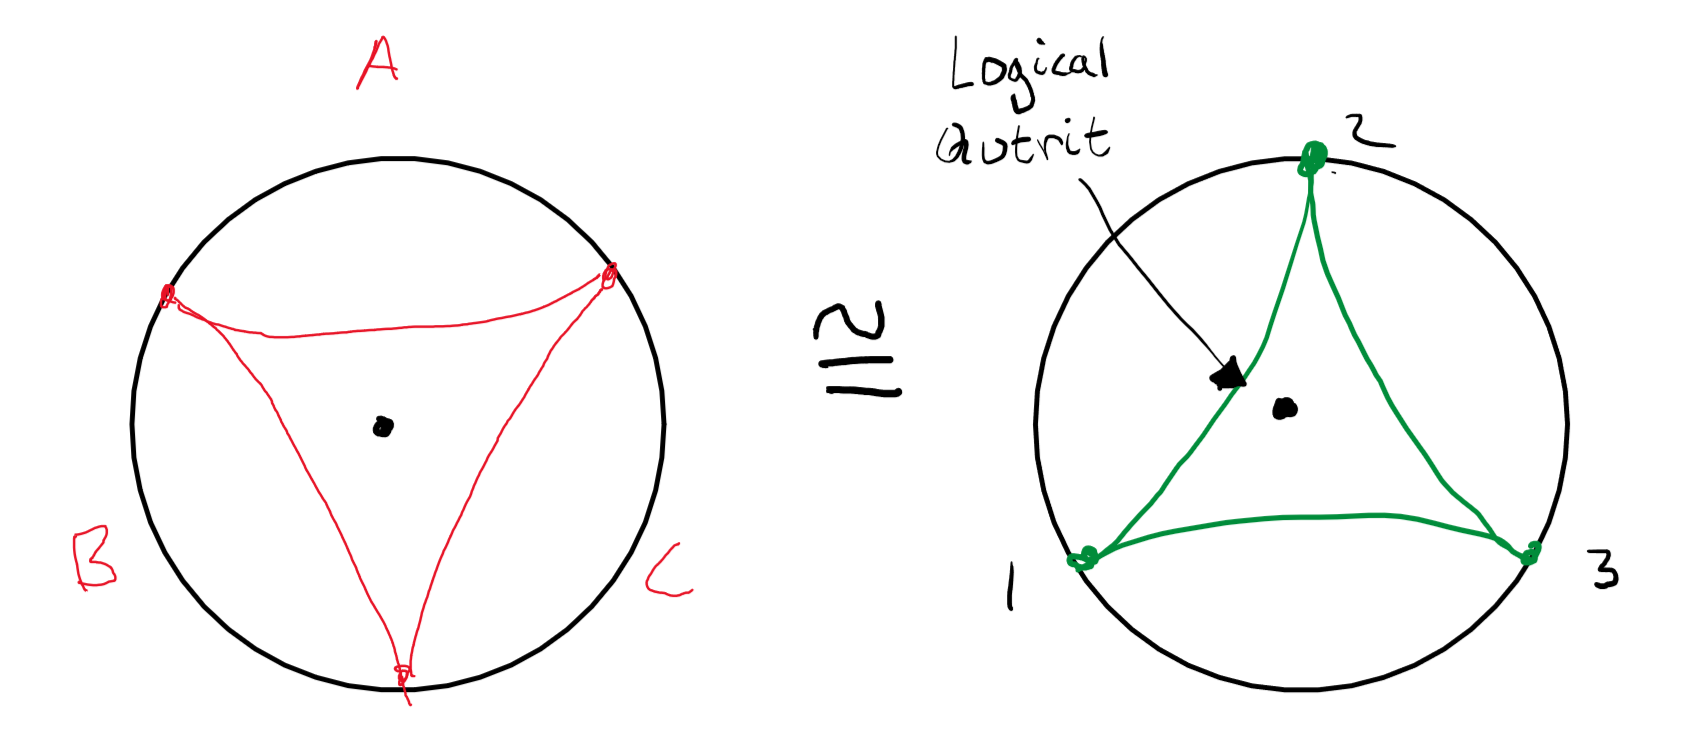
\includegraphics[width=0.95\linewidth]{ADS_CFT_Fig5}
	\caption{}
	\label{fig:adscftfig5}
\end{figure}
Further, in this setup \eqref{eq:2} only has support when states lie in $H_{\text{code}}$, where the code subspace are defines as states that are perturbatively close to the vacuum.
\begin{equation}
	\begin{aligned}
		\langle \tilde \psi |\left[\phi(x),\BO(X)\right]|\tilde \psi\rangle =0,~~~~~~~~\forall~~~~ |\tilde \psi\rangle\in H_{\text{code}}
	\end{aligned}
\end{equation}
\begin{figure}[]
	\centering
	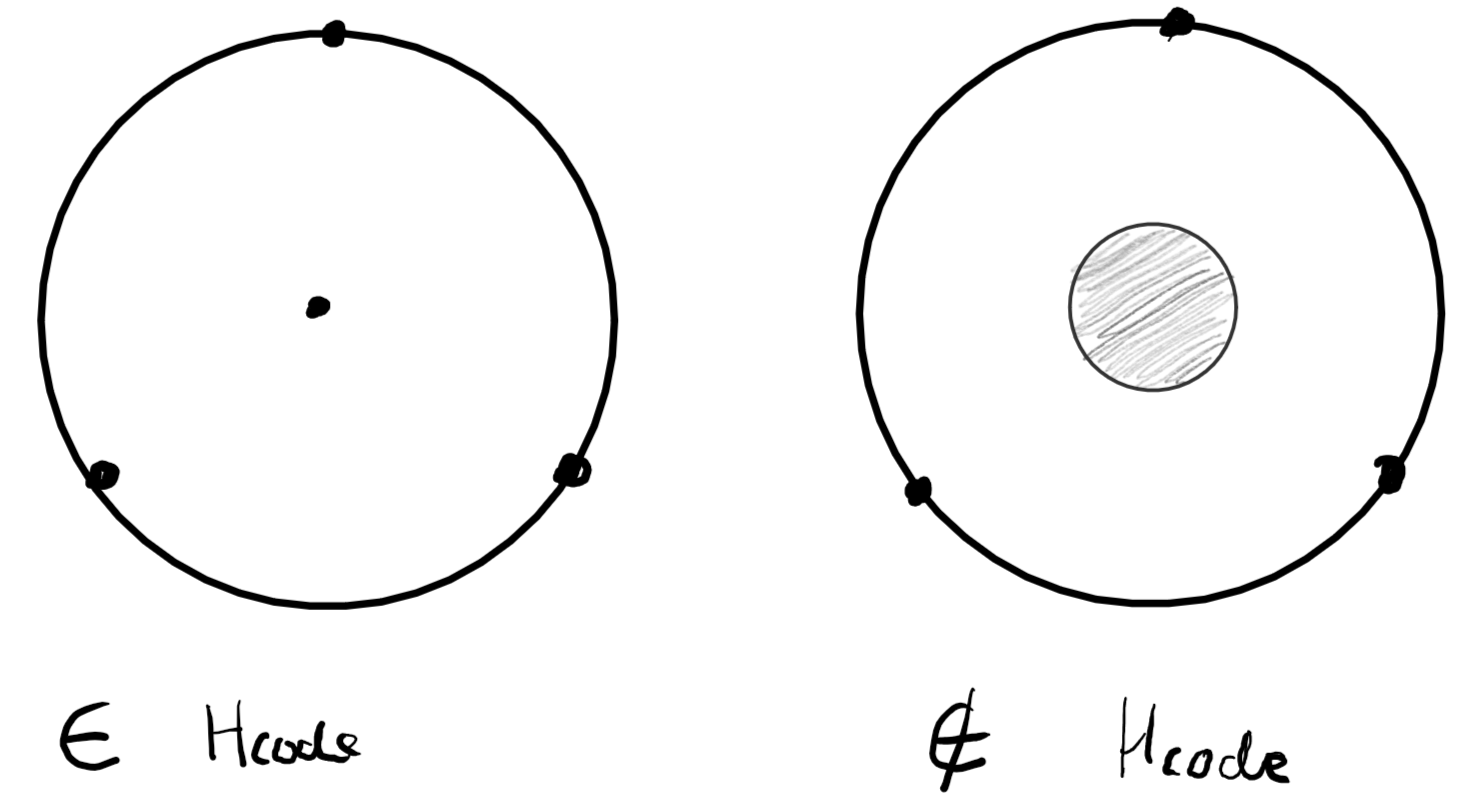
\includegraphics[width=0.7\linewidth]{ADS_CFT_Fig6}
	\caption{}
	\label{fig:adscftfig6}
\end{figure}
\section{Tensor Models}
\section{Outlook}
%%%%%%%%%%%%%%%%%%%%%%%%%%%%%%
%%%%%%%%%%%%%%%%%%%%%%%%%%%%%%
%%%%%%%%%%%%%%%%%%%%%%%%%%%%%%
%%%%%%%%%%%%%%%%%%%%%%%%%%%%%%
%%%%%%%%%%%%%%%%%%%%%%%%%%%%%%
%%%%%%%%%%%%%%%%%%%%%%%%%%%%%%
%%%%%%%%%%%%%%%%%%%%%%%%%%%%%%
%%%%%%%%%%%%%%%%%%%%%%%%%%%%%%
%%%%%%%%%%%%%%%%%%%%%%%%%%%%%%
\newpage
\begin{thebibliography}{99}
%\cite{Arkani-Hamed:2010zjl}
\bibitem{amp1}
N.~Arkani-Hamed, J.~L.~Bourjaily, F.~Cachazo, S.~Caron-Huot and J.~Trnka,
%``The All-Loop Integrand For Scattering Amplitudes in Planar N=4 SYM,''
JHEP \textbf{01}, 041 (2011)
doi:10.1007/JHEP01(2011)041
[arXiv:1008.2958 [hep-th]].
%411 citations counted in INSPIRE as of 10 Oct 2021
%\cite{Elvang:2015rqa}
\bibitem{Elvang}
H.~Elvang and Y.~t.~Huang,
``Scattering Amplitudes in Gauge Theory and Gravity,''
%18 citations counted in INSPIRE as of 10 Oct 2021
%\cite{Arkani-Hamed:2012zlh}
%393 citations counted in INSPIRE as of 10 Oct 2021
%\cite{Arkani-Hamed:2013jha}
\bibitem{amp3}
N.~Arkani-Hamed and J.~Trnka,
%``The Amplituhedron,''
JHEP \textbf{10}, 030 (2014)
doi:10.1007/JHEP10(2014)030
[arXiv:1312.2007 [hep-th]].
%352 citations counted in INSPIRE as of 10 Oct 2021
%\cite{Arkani-Hamed:2013kca}
\bibitem{amp4}
N.~Arkani-Hamed and J.~Trnka,
%``Into the Amplituhedron,''
JHEP \textbf{12}, 182 (2014)
doi:10.1007/JHEP12(2014)182
[arXiv:1312.7878 [hep-th]].
%133 citations counted in INSPIRE as of 10 Oct 2021
\bibitem{amp6}
N.~Arkani-Hamed, A.~Hodges and J.~Trnka,
%``Positive Amplitudes In The Amplituhedron,''
JHEP \textbf{08}, 030 (2015)
doi:10.1007/JHEP08(2015)030
[arXiv:1412.8478 [hep-th]].
%70 citations counted in INSPIRE as of 10 Oct 2021
\bibitem{on1}
N.~Arkani-Hamed, J.~L.~Bourjaily, F.~Cachazo, A.~Postnikov and J.~Trnka,
%``On-Shell Structures of MHV Amplitudes Beyond the Planar Limit,''
JHEP \textbf{06}, 179 (2015)
doi:10.1007/JHEP06(2015)179
[arXiv:1412.8475 [hep-th]].
%68 citations counted in INSPIRE as of 10 Oct 2021
%\cite{Herrmann:2016qea}
\bibitem{amp2}
N.~Arkani-Hamed, J.~L.~Bourjaily, F.~Cachazo, A.~B.~Goncharov, A.~Postnikov and J.~Trnka,
%``Grassmannian Geometry of Scattering Amplitudes,''
doi:10.1017/CBO9781316091548
[arXiv:1212.5605 [hep-th]].
\bibitem{on2}
E.~Herrmann and J.~Trnka,
%``Gravity On-shell Diagrams,''
JHEP \textbf{11}, 136 (2016)
doi:10.1007/JHEP11(2016)136
[arXiv:1604.03479 [hep-th]].
%42 citations counted in INSPIRE as of 10 Oct 2021
%\fi
\end{thebibliography}
\end{document}

